% !TeX program = xelatex
% !TeX encoding = utf8

\documentclass[]{article}

\usepackage{fontspec}
\setmainfont{Garamond}

\usepackage{textcomp}

\usepackage{hyperref}

\usepackage{fancyhdr}
\pagestyle{fancy}
\fancyhf{} % sets both header and footer to nothing
\renewcommand{\headrulewidth}{0pt}
\rfoot{\textcopyright Project Meta-Management}
\cfoot{\thepage}

\title{Phase 1: Definition}
\author{ \begin{tabular}{rl}
		\textbf{Team Leader:} & Preston Engstrom \\
		\textbf{Working Group:} & Tyler Kennedy Collins\\ & Yucen Jin \\ & Jaclyn Binch  \\ & Andrew Rooney \\ & Jeff Yang \\ & Alex Lawrence
	\end{tabular}}
\date{}
	
\begin{document}

\maketitle

\thispagestyle{fancy}

\abstract
This document describes the definition phase of Homestead. Homestead is a web application that provides services in the area of rental, sublet searching, and posting for tenants as well as landlords.

\section{Context}
As attitudes and economic changes occur, more of the adult population is shifting their focus away from home ownership towards renting. This reality, combined with web applications becoming ubiquitous create a market for Homestead. \\Homestead provides an effective service by offering landlords a simple and easy way to effectively list their available properties. For tenants, Homestead offers custom searching, alerts to mobile devices, reviews of landlords via a comments section, and a way to view past listings.

\section{Objectives}
The primary goal of the project is to create an attractive, stable, and scalable web service which, upon completion can rapidly be turned into a functional business. The web application will present a platform to allow for the advertisement, searching and viewing of rental properties including student housing and sublets. The application will provide varied interfaces to serve two client groups: landlords and tenants. Tenants will be able to search for postings via user specified criteria or by using a map interface. Tenants will be able to review comments from previous tenants regarding the landlord or property. Landlords will conversely be provided with an interface to create and edit property postings. This type of user will also possess the capability to interact and vet potential tenants. Finally, landlords will be able to view metrics on other posting to stay competitive. Users will be able to save searches for a particular area so as to monitor when a suitable posting becomes available. This user will be notified of postings meeting their criteria via SMS or email, based on their preferred communication method as detailed within their profile.

\section{Features}
\begin{itemize}
	\item Mapping and Geo-location service.
	\item Video streaming service for viewing rooms.
	\item Street level view through the Google Maps API.
	\item Cross platform support.
	\item System to evaluate and rank postings given a set of criteria.
	\item Automated interaction with users via SMS and email.
	\item Persistent instant messaging service to support direct communication of tenant and landlord users via Homestead.
	\item Commenting and rating system for tenants and landlords.
	\item Simple, interactive, and easy to use searching interface for listings.
\end{itemize}

\section{Implementation Requirements}
\begin{itemize}
	\item Web server with LAMP stack (Linux, Apache, MySQL, PHP) for testing and deployment.
	\item Google Developer account/Access to Google API's.
	\item Software and hardware infrastructure for sending SMS messages.
	\item Properties/Interior images to use as preliminary test data.
	\item Front and back end development frameworks to avoid creation of solutions to previously solved problems. \textbf{See Below}
\end{itemize}
\subsection{Use of Frameworks in Development}
Programming frameworks provide a set of pre-built tools and components to avoid "reinventing the wheel". Many open source frameworks exist for a multitude of languages. For our purposes, we have selected two frameworks, to be discussed in sections 5.1 and 5.2.

\section{Development Environment}
Our development team will be working on a variety of platforms for local development, testing and production fixes. To avoid cross-platform compatability issues, we have standardized the environments we are using. This section gives an overview of our frameworks and environments.
\subsection{Front End Framework: Bootstrap}
The front end of the application will be built by extending the Bootstrap front end framework. Bootstrap is an open source collection of CSS classes to be applied on website elements. The primary goal of Bootstrap is to provide developers with the ability to create websites that are responsive. An example would be to adapt to varying screen sizes.
\subsection{Back End Framework: Laravel 5.2}
Laravel is a PHP framework that provides standard classes and stable systems for interacting with databases. Creating front end templates that are otherwise simple but tedious to build reinforces our framework design decision. By using a framework that provides standard features, such as user authentication through Google, Facebook, and Twitter, it allows the development team to focus on significantly more advanced problems. These include full support of mobile platforms, a more responsive website, and integration of SMS sending.
\subsection{Local Development}
Team members will be developing on a variety of platforms. To maintain consistency throughout the process, all development will take place on virtual machines. Each team member will have an identical machine, hosted using Oracle Virtualbox, allowing team members to develop in an environment matching the production set up. This provides consistency regardless of the developers physical platform. This is advantageous as team members are developing on Microsoft Windows, Apple OSx and a variety of Linux OS distributions.

\section{Source Control}
All source code, documentation, business documents, meeting minutes, and other pertinent information will be maintained via the Git version control system.
\subsection{Git Project Name Selection}
Project names are often overlooked as an important part of a team development environment. As the software development industry has grown, large corporations and small startups alike have begun to converge on the idea of fostering a comfortable work environment. By generating project names that seem nonsensical, but memorable, teams also foster a more cohesive environment. To this end, the team has elected to randomly generate a project name. The selected name is \textbf{Barbaric Waffle}. This name achieves the memorability and approachability that other companies, including Google, Facebook and Twitter, strive towards for in their development projects.

\section{Acceptance Criteria}
The criteria found below make up the minimum acceptance level for the application to be considered completed.
\begin{enumerate}
	\item Application must be built to a point that it is ready to be deployed in a business environment.
	\item The application will present a usable, modern interface across all platforms.
	\item Support for a mobile client must exist. This can take the form of a web application.
	\item Users will be able to view listings made by landlords.
	\item Information regarding listings will have criteria for location, amenities, and more.
	\item Listings will be indexable for criteria and via a map interface.
	\item Tenants will be able to view previously viewed listings.
	\item User must be able to receive alerts regarding creation of new pertinent listings.
\end{enumerate}

\section{Personnel Roles}
All team members will take up general programming and documentation roles, combined with their designated roles. All team members will participate in regular bi-weekly code reviews and interface reviews.
\subsection{Team Leader}
The team leader serves as the Chief Designer, Senior Programmer, and Chief Technical Manager. They are responsible for analysis and design, source control, data control, reviews, user documentation, writing critical source components, and assigning work to other team members.
\subsection{Deputy Leader}
The Deputy Leader shares all roles of the Team Leader. The Deputy Leader is also ready at any time to take  over as the Team  Leader.
\subsection{Test Leader}
Responsible for overseeing application testing. Provides first review of all changes before moving from development to staging environment. Is prepared to take over at any time as Deputy Leader.
\subsection{Test Programmer}
Collaborates with Test Leader in developing test cases and testing builds.
\subsection{Technical Librarian}
Maintains documentation library. Prepares input data, cares for server infrastructure, and meeting minutes.
\subsection{Technical Writer}
Assists Team Leader in preparation of documentation, support documents, phase documents, and reports.
\subsection{General Programmer}
Responsible for detailed design and programming of front and back end components.

\subsection{Team Testing Structure}
Testing of features will be done by all team members, excluding the member responsible for the development of that feature. It should be noted that the goal of this structure is to allow members to receive constructive criticism from the group as a whole so that all members can learn from what is properly implemented. This is to avoid repeated mistakes.
\section{Team Members}
\begin{itemize}
	\item \textbf{Tyler Kennedy Collins} Deputy Leader
	\item \textbf{Jaclyn Binch} Technical Writer / Test Programmer
	\item \textbf{Yucen Jin} Technical Librarian / Test Programmer
	\item \textbf{Jeff Yang} General Programmer / Technical Writer
	\item \textbf{Alex Lawrence} Test Leader / Test Programmer
	\item \textbf{Andrew Rooney} General Programmer / Technical Writer
	\item \textbf{Preston Engstrom} Team Leader / Technical Writer
\end{itemize}

\section{Team Organization}
The project will follow the Agile SCRUM development methodology. Development will be broken into 3 groups: Front End, Back End and Database. Each group will deal with an equally critical segment of development. All three groups will meet together at bi-weekly meetings. Each group will then meet separately, directly after each team meeting.

\section{Preliminary Design}
%%% INCLUDE THE SITE MAP with descriptions of functions on major pages
The project's preliminary design is focused on how a user will traverse the application. By defining the site map first, it allows both the Front End and Back End development teams to identify priority interfaces and services.\\
\begin{center}
	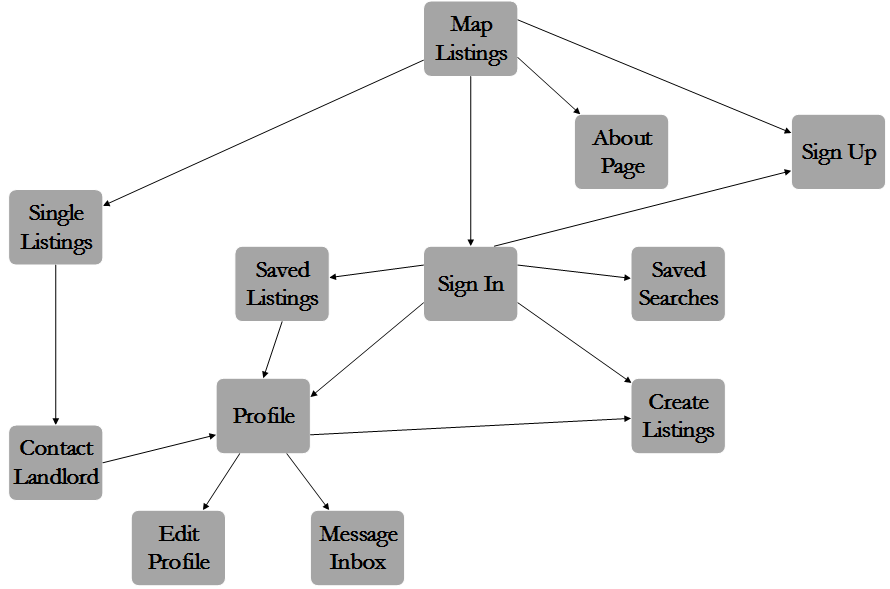
\includegraphics[width=0.75\textwidth]{Phase1SiteMap.png}
\end{center}
\\
A more expanded design document will be presented to the customer upon approval of the Definition document. This design document will include the data flow diagrams, database schema diagrams, interface mock-ups and Agile User Stories.

\end{document}
